\section{Progettazione}

\subsection{Design Persona}

Partendo dalla risorsa consigliata nel corso (\textit{Desining for Emotion} di
Aaron Walter), abbiamo descritto la personalità di partenza per sviluppare il
prodotto:

\begin{itemize}
	\item \textbf{Brand name}: \textit{Grigo Verde}. Il nome è stato scelto per
	      richiamare il nome della scuola abbinato al colore verde, che richiama
	      gli spazi all'aperto e la natura;

	\item \textbf{Overview}: il sito prosegue il lavoro degli studenti del Liceo
	      Grigoletti che hanno partecipato ad un progetto di riqualificazione
	      delle aree verdi della scuola. Per questo motivo il verde è il colore
	      predominante del sito ed è prensente anche nel nome;

	\item \textbf{Brand traits}:
	      \begin{itemize}
		      \item Formale ma non rigido: deve essere adatto ad un contesto
		            scolastico;

		      \item Semplice e banale: considerando il target del sito, è
		            fondamentale che sia facile da usare e che non ci siano
		            elementi che possano confondere l'utente;

		      \item Preciso: deve essere sempre pronto a rispondere ad ogni
		            esigenza dell'utente con la massima accuratezza;

		      \item Accattivante, ma non complesso: la scelta dei colori è
		            stata fatta in parte con il proponente del progetto, un
		            insegnante di arte, per garantire un impatto visivo
		            accattivante, senza però appesantire il sito.
	      \end{itemize}

	\item \textbf{Personality map}:
	      \begin{center}
		      \begin{tikzpicture}
			      \begin{axis}[
					      axis lines = middle,
					      xlabel = { semplice },
					      ylabel = { formale },
					      xmin = -11, xmax = 11,
					      ymin = -11, ymax = 11,
					      xtick = {-10,-5,...,10},
					      ytick = {-10,-5,...,10},
					      xlabel style={at={(ticklabel cs:1)}, anchor=north},
				      ]
				      % template per mostrare il punto all'interno del piano cartesiano.
				      \addplot [
					      color=black,
					      mark=*,
					      only marks,
				      ] coordinates {
						      (10, 3)
					      } node[below] {$P$};
			      \end{axis}
		      \end{tikzpicture}
	      \end{center}

	      Si noti che si tratta più che altro dell'aspettativa che vogliamo
	      raggiungere, non è detto che siamo stati in grado di raggiungere 10 in
	      semplicità. Tuttavia, vogliamo chiarire che la semplicità è il nostro
	      obiettivo principale;

	\item \textbf{Visual lexicon}:
	      \begin{itemize}
		      \item \textbf{Colori}: verde scuro per i titoli, nero per i testi
		            e bianco per lo sfondo. Ogni tanto ci sono delle decorazioni
		            rosse per attirare l'attenzione dell'utente e per richiamare
		            il colore della scuola;

		      \item \textbf{Contorni}: i contorni arrotondati rendono il
		            prodotto più accattivante e diminuiscono il senso di rigidità
		            e il carico cognitivo;

		      \item \textbf{Font}: \textit{Sans-Serif Arial};
	      \end{itemize}

	\item \textbf{Engagement methods}:
	      \begin{itemize}
		      \item \textbf{Design intuitivo}: l'utente deve essere in
		            grado di capire cosa fare senza dover leggere alcun manuale;

		      \item \textbf{Psicologia dei colori}: sono utilizzati dei colori
		            accattivanti che richiamano il verde della natura;

		      \item \textbf{Feedback}: l'utente deve ricevere un feedback
		            ad ogni azione che compie, in modo da rassicurarlo e
		            mantenere il suo interesse, evitando frustrazioni.
	      \end{itemize}
\end{itemize}

\subsection{Palette}

La palette di colori è stata scelta in base alla personalità del brand;
infatti sono stati selezionati con un contrasto elevato tra loro in
modo da garantire una buona leggibilità anche da parte di utenti con deficit
parziale della vista.
Non solo, ci siamo assicurati che colori simili non fossero accostati in modo
da evitare confusione tra di essi. Di seguito evidenziamo la palette di colori.

\begin{itemize}
	\item Sfondo: \#ffffff;
	\item Colore del testo: \#333333;
	\item Colore primario: \#335833;
	\item Colore secondario: \#0000ff;
	\item Colore terziario: \#73dec1;
	\item Colore per gli errori: \#e22c2f;
\end{itemize}

\begin{figure}[h]
	\label{fig:palette}
	\centering
	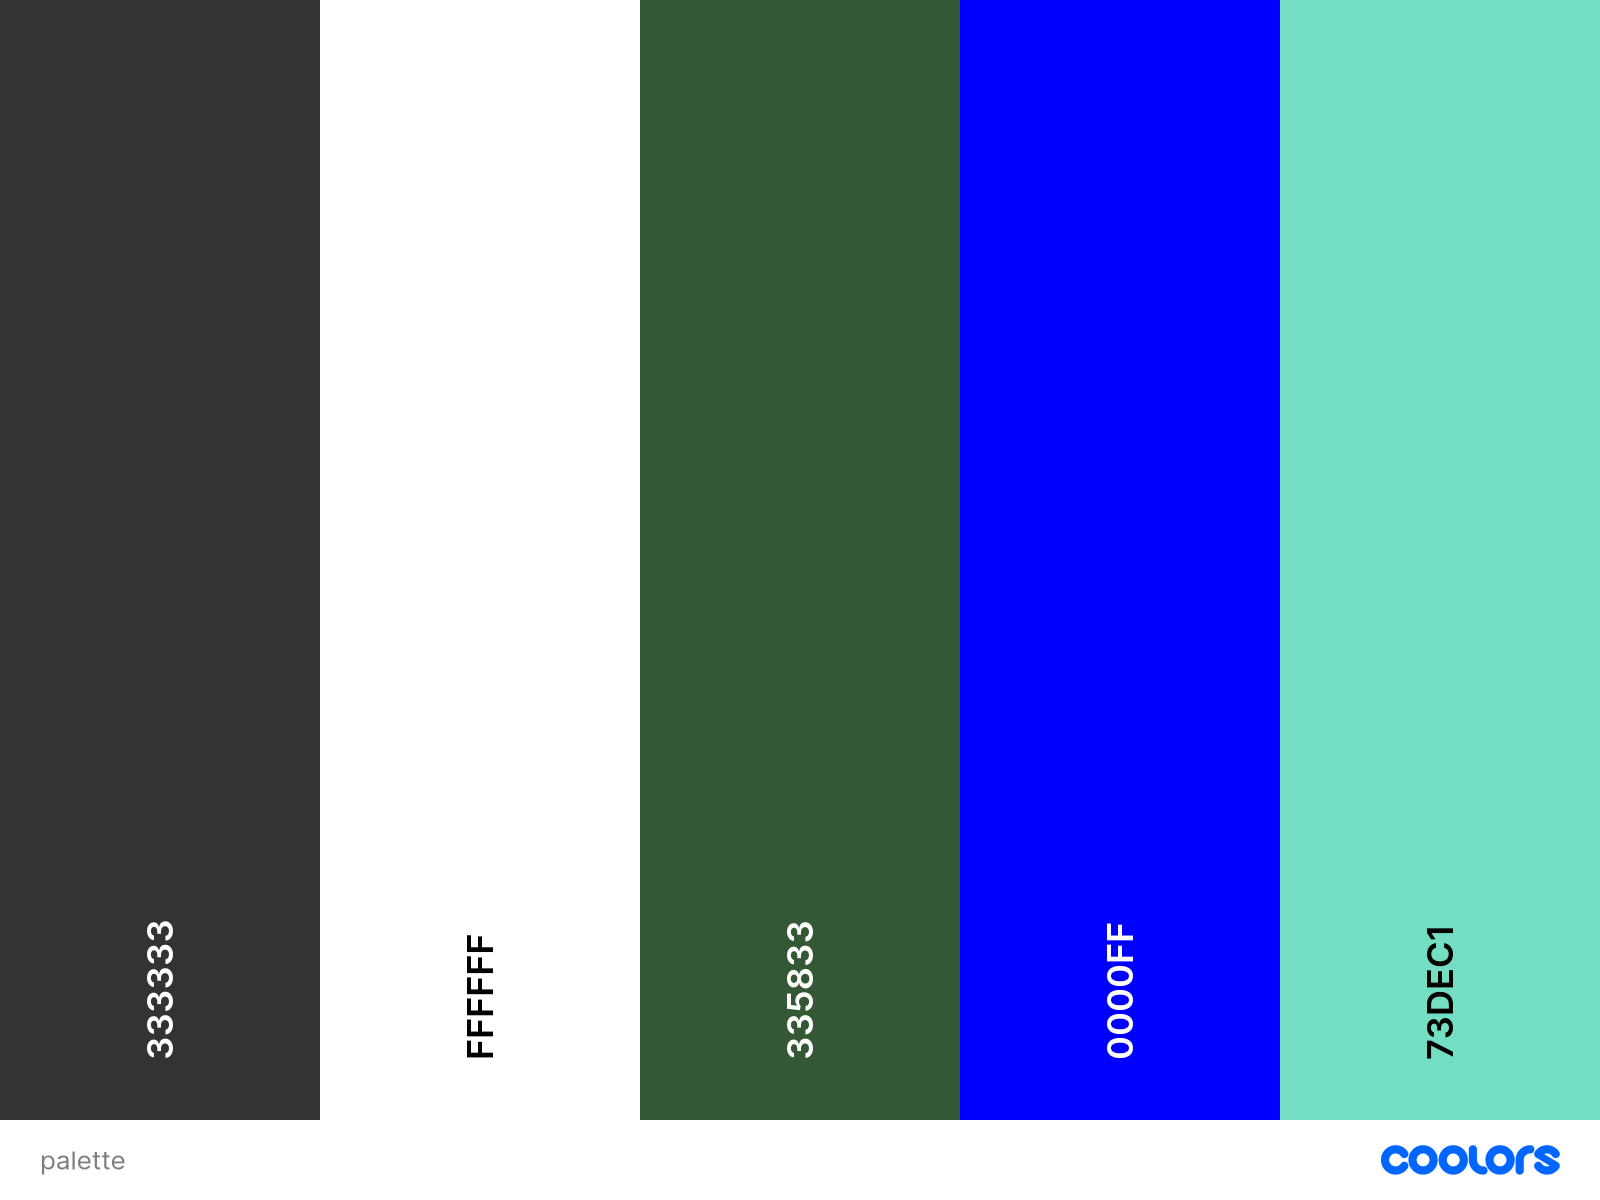
\includegraphics[width=0.8\textwidth]{figures/palette.png}
	\caption{Palette di colori scelta per il sito.}
\end{figure}

In particolare abbiamo prestato attenzione alle seguenti coppie di contrasto:
\begin{itemize}
	\item sfondo e testo;

	\item sfondo e colore primario: il colore primario è usato per l'header,
	      il footer, i link visitati e per i titoli, mentre lo sfondo è usato
	      per il testo nell'header e nel footer e come sfondo nel resto del
	      sito;

	\item sfondo e colore secondario: il colore secondario è usato per i link
	      non visitati, considerando il target di utenza, è stato scelto un
	      blu accesso, uno standard per questo tipo di link;

	\item colore primario e terziario: pensavamo di usare il colore
	      terziario per segnalare i link all'interno dell'header,
	      tuttavia per evitare sovraccarichi visivi, abbiamo optato per
	      usare il colore dello sfondo sia per il testo che per i link
	      all'interno dell'header.
	      Dunque il colore terziario è stato usato per alternare le righe
	      delle tabelle, in modo da facilitarne la lettura;

	\item sfondo e colore per gli errori: il colore per gli errori è usato
	      per evidenziare i form che sono stati compilati in modo improprio e
	      per spiegare in quale modo correggere le informazioni inserite.
	      Questo colore è stato scelto per contrastare con lo sfondo bianco
	      in modo da attirare l'attenzione dell'utente e facilitare la
	      correzione. Questo colore è usato anche in modo decorativo per
	      rendere il sito più accattivante;

	\item colore secondario e terziario: questi due colori si sovrappongono
	      all'iterno delle tabelle, dove sono presenti i link per andare al
	      dettaglio di una prenotazione.
\end{itemize}

Il contrasto più basso tra queste coppie risulta essere tra il colore primario
e il colore terziario, con un rapporto di 5.01:1, che rispetta comunque lo
standard WCAG AA anche per un testo di dimensione inferiore a 17pt.

\subsection{Accessibilità}

L'accessibilità è un indice di qualità del sito, pertanto è stata fin da subito
un proposito imprescindibile che ha guidato la fase di progettazione e le
successive. Di seguito sono riportate le misure adottate per garantire
un'esperienza di utilizzo ottimale per tutti gli utenti.

\subsubsection{Orientamento dell'utente}

Per garantire un'esperienza di utilizzo ottimale e ridurre il disorientamento e
il sovraccarico cognitivo, sono state adottate diverse misure:

\begin{itemize}
	\item \textbf{Breadcrumb}: utilizzo di breadcrumb in ogni pagina per
	      facilitare la navigazione e mantenere l'utente consapevole della
	      propria posizione all'interno del sito;

	\item \textbf{Link circolari}: controllo rigoroso nella costruzione della
	      pagina per evitare la presenza di link circolari che potrebbero
	      confondere l'utente;

	\item \textbf{Link}: tutti i link sono sottolineati e i link non visitati
	      hanno il classico blu, mentre i link visitati sono di colore verde
	      scuro. L'unica eccezione è il logo il logo del sito in alto a sinistra
	      che è un link che riporta alla home. Tuttavia, all'interno del menù è
	      presente il collegamento alla home, quindi non riteniamo che possa
	      creare confusione;

	\item \textbf{Vai al contenuto}: implementazione della funzionalità "vai al
	      contenuto" per migliorare l'accessibilità agli utenti che utilizzano
	      screen reader oppure che navigano dal telefono;

	\item \textbf{Torna su}: aggiunta del pulsante "torna su" alla fine di
	      ogni pagina, che diventa visibile scorrendo verso il basso,
	      facilitando così il ritorno rapido all'inizio della pagina stessa.
	      Il pulsante non è visibile negli schermi grandi;

	\item \textbf{Linguaggio semplice}: abbiamo adottato un linguaggio adatto al
	      target di utenza; per esempio, all'inizio avevamo usato il termine
	      "dashboard" per indicare la homepage di un utente autenticato, tuttavia
	      ci siamo resi conto che poteva creare confusione, quindi abbiamo
	      cambiato il termine in "cruscotto";

	\item \textbf{Alternative testuali}: tutte le immagini hanno un'alternativa
	      testuale che permetta di comunicare il contenuto dell'immagine a chi
	      non è in grado di vederla;

	\item \textbf{Attributo \texttt{lang}}: l'attributo \texttt{lang} è stato
	      aggiunto in ogni pagina per indicare la lingua principale del sito,
	      in modo da permettere agli screen reader di selezionare la voce
	      corretta per la lettura del testo, inoltre è stato aggiunto anche
	      ad ogni parola o frase in lingua straniera;

	\item \textbf{Tag \texttt{time}}: il tag \texttt{time} è stato utilizzato
	      per indicare date e orari, in modo da permettere agli screen reader
	      di leggere correttamente queste informazioni;

	\item \textbf{Tabelle accessibili}: le tabelle sono state progettate in modo
	      da essere accessibili, secondo le indicazioni approfondite durante il
	      corso;

	\item \textbf{Tag \texttt{aria-label} e \texttt{aria-describedby}}: dove
	      necessario, sono stati aggiunti attributi \texttt{aria-label} e
	      \texttt{aria-describedby} per comunicare informazioni aggiuntive agli
	      screen reader;

	\item \textbf{Creazione e rispetto di convenzioni interne al sito}.
\end{itemize}

\subsubsection{Responsive layout}

Il sito è stato progettato per adattarsi a qualsiasi dispositivo, in modo da
garantire un'esperienza di utilizzo ottimale sia da desktop che da mobile. Per
questo motivo, sono stati adottati layout flessibili e fluidi, in modo da
garantire una buona leggibilità e usabilità indipendentemente dalla dimensione
dello schermo o dalle preferenze dell'utente: infatti abbiamo utilizzato solo
unità di misura proporzionali come \texttt{em} oppure \texttt{\%}, tranne che
per la dimensione minima delle schede che mostrano uno spazio, che è stata
impostata a 150px, per garantire una buona visualizzazione delle immagini.\\
I breakpoint sono stati scelti
con cura per garantire una transizione fluida tra i diversi layout e una
buona esperienza di utilizzo su tutti i dispositivi. Sono rispettivamente:
\begin{itemize}
	\item minore di 700: layout mobile, per telefoni e piccoli schermi;

	\item tra 701 e 900px: layout tablet, per tablet e schermi di dimensioni
	      medie;

	\item tra i 901px e i 1223px: layout desktop, per schermi di dimensioni
	      medie e per i tablet in modalità landscape;

	\item maggiore di 1224px: layout desktop, per schermi di grandi dimensioni.
\end{itemize}

In realtà, dato che abbiamo delle tabelle piuttosto larghe, abbiamo introdotto
dei breakpoint aggiuntivi per garantire un layout dinamico a partire dai
300px.\\
Infine, per la pagina "About us" abbiamo aggiunto un breakpoint a 1024px per
cambiare il layout della pagina in modo da garantire una migliore leggibilità
e evitare che l'utente si stanchi di leggere un testo troppo lungo.

\subsection{Struttura del sito}

Abbiamo cominciato a progettare il sito partendo da un'analisi delle esigenze e
quindi delle funzionalità che il sito deve offrire. Abbiamo quindi definito
l'elenco delle pagine che compongono il sito e abbiamo diviso le funzionalità
all'interno di queste pagine.
Abbiamo individuato funzionalità comuni a più pagine e le abbiamo raggruppate.
Infine abbiamo collegato le pagine tra loro in modo da definire un percorso
di navigazione logico e intuitivo per l'utente.
Finalmente abbiamo definito la struttura organizzativa del sito, ovvero la
mappa del sito: abbiamo deciso di adottare la struttura gerarchica per garantire
maggiore chiarezza e facilità di navigazione all'utente.\\
Per evitare il rischio del sovraccarico cognitivo, abbiamo deciso di includere 4
voci nel menù principale, in modo da garantire all'utente un accesso rapido alle
pagine principali del sito. Se l'utente effettua il login come docente allora
viene aggiunta la voce "cruscotto" al menù; se l'utente effettua il login come
amministratore allora viene aggiunta anche la voce "utenti". In questo modo il
menù del sito ha un numero di voci variabile da 4 a 6. Infine il sito ha una
profondità di 4 livelli; in questo modo l'utente può raggiungere qualsiasi
pagina in massimo 3 click, più due se l'utente deve effettuare il login.

\begin{figure}[h]
	\centering
	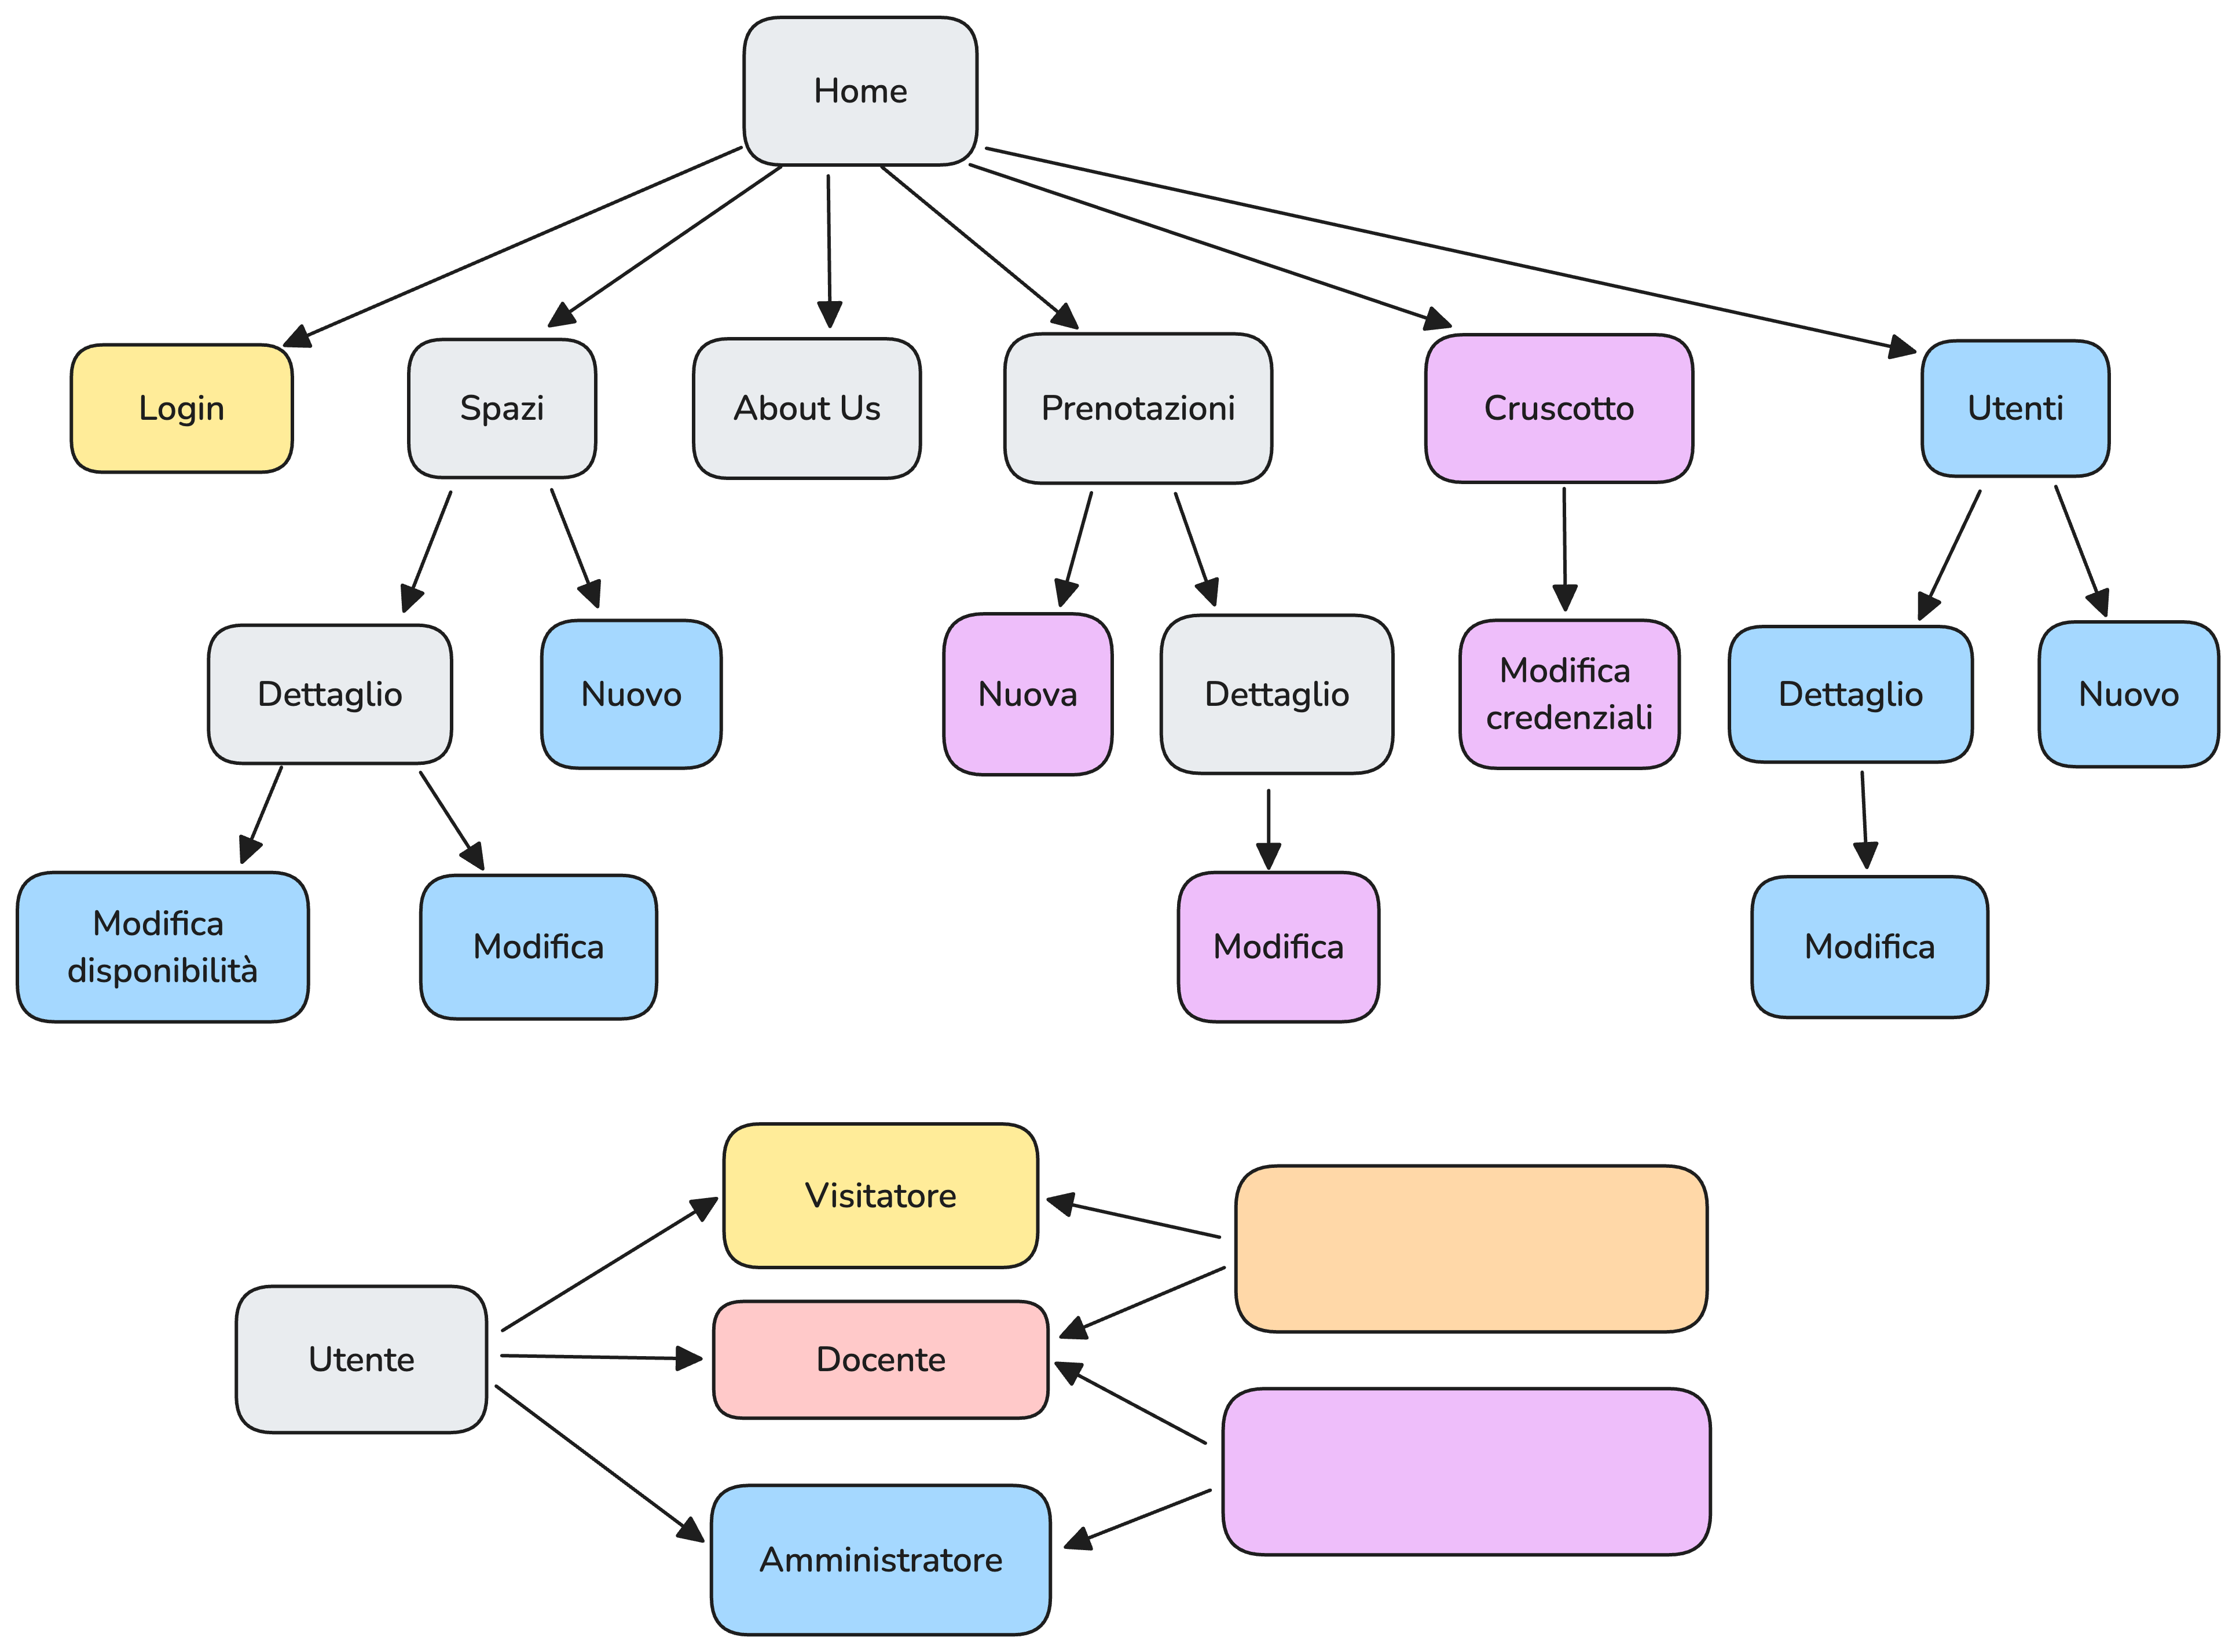
\includegraphics[width=0.8\textwidth]{figures/sitemap.png}
	\caption{Mappa del sito sopra e legenda dell'accesso alle pagine sotto.}
\end{figure}

Di seguito sono descritte le pagine del sito:

\begin{itemize}
	\item \textbf{Homepage}: in genere è la prima pagina che viene visualizzata
	      quando si accede al sito Grigo Verde. Contiene una breve descrizione
	      del progetto e delle funzionalità disponibili;

	\item \textbf{Login}: pagina di autenticazione al sito;

	\item \textbf{About us}: pagina che contiene informazioni sul progetto in
	      dettagliato, spiegando come è nato e quali sono gli obiettivi;

	\item \textbf{Cruscotto}: pagina di benvenuto per gli utenti autenticati,
	      contiene il riepilogo delle prenotazioni future o in corso dell'utente
	      oltre che alle azioni rapide che l'utente può compiere;

	      \begin{itemize}
		      \item \textbf{Modifica credenziali}: pagina per modificare le
		            credenziali dell'utente autenticato, compresa la password;

		      \item \textbf{Nuovo Spazio}: un amministratore può accedere a
		            questa pagina per creare un nuovo spazio.

		      \item \textbf{Nuova prenotazione}: si accede a questa pagina per
		            effettuare una nuova prenotazione. Si noti che un
		            riferimento a questa pagina è prensente anche nel dettaglio
		            di uno spazio e nel cruscotto dell'utente autenticato.

		      \item \textbf{Nuovo utente}: si accede a questa pagina per
		            registrare un nuovo utente all'interno del sistema.
	      \end{itemize}

	\item \textbf{Spazi}: pagina di visualizzazione degli spazi verdi della
	      scuola e delle aree ricreative, è possibile filtrare gli spazi;

	      \begin{itemize}
		      \item \textbf{Dettaglio di uno spazio}: sono visualizzate le
		            informazioni relative ad uno spazio, come il nome,
		            l'immagine o anche le prenotazioni e gli orari di apertura
		            dello stesso. Non solo, se l'utente è autenticato, allora
		            può accedere alla pagina di prenotazione direttamente da
		            qui;

		            \begin{itemize}
			            \item \textbf{Modifica spazio}: pagina per modificare le
			                  informazioni di uno spazio;

			            \item \textbf{Modifica orari di apertura}: pagina per
			                  modificare gli orari di apertura di uno spazio.
		            \end{itemize}
	      \end{itemize}

	\item \textbf{Prenotazioni}: pagina di visualizzazione delle prenotazioni
	      future registrate nel sistema;

	      \begin{itemize}
		      \item \textbf{Dettaglio di una prenotazione}: sono visualizzate le
		            informazioni relative ad una prenotazione, l'orario della
		            prenotazione, lo spazio prenotato e l'utente che ha
		            effettuato la prenotazione. Se l'utente è autenticato e ha
		            effettuato la prenotazione oppure è un amministratore,
		            allora può cancellare o modificare la prenotazione
		            direttamente da qui;

		            \begin{itemize}
			            \item \textbf{Modifica prenotazione}: pagina per
			                  modificare le informazioni di una prenotazione;
		            \end{itemize}
	      \end{itemize}

	\item \textbf{Utenti}: pagina di visualizzazione degli utenti registrati nel
	      sistema. Si noti che questa pagina è accessibile solo agli
	      amministratori, lo stesso vale per le pagine qui sotto;

	      \begin{itemize}
		      \item \textbf{Dettaglio di un utente}: sono visualizzate le
		            informazioni relative ad un utente, oltre che alle sue
		            prenotazioni future;

		            \begin{itemize}
			            \item \textbf{Modifica di un utente}: pagina per
			                  modificare le informazioni di un utente compresa
			                  la password.
		            \end{itemize}
	      \end{itemize}
\end{itemize}

\subsection{SEO}

Innanzitutto, abbiamo immaginao il \textit{search intent} dei nostri utenti.
Abbiamo identificato le seguenti \textit{query} che potrebbero essere
utilizzate per cercare il nostro sito:
\begin{itemize}
	\item \textbf{Grigo Verde};
	\item \textbf{Liceo Grigoletti};
	\item \textbf{Liceo Scientifico Pordenone};
	\item \textbf{Spazi verdi};
	\item \textbf{Aule all'aperto};
\end{itemize}

A partire da queste \textit{query}, abbiamo scritto i tag \texttt{<title>},
\texttt{<meta name="description">} e \texttt{<meta name="keywords">} delle
pagine del nostro sito. Si noti, che queste informazioni non sono aggiunte alle
pagine che richiedono l'autenticazione, in quanto non sono indicizzate dai
motori di ricerca e non sono accessibili ai visitatori non autenticati. In
aggiunta, sono state aggiunte keyword specifiche per ogni pagina, in modo da
migliorare il posizionamento nei motori di ricerca.\\
Finalmente, sono state adottate soluzioni tecniche, come la
divisione tra la struttura, la presentazione ed il comportamento per ridurre il
peso delle pagine e migliorare il \textit{ranking} nei motori di ricerca. Le
soluzioni tecniche adottate sono spiegate nel dettaglio nelle sezioni dedicate.
